\documentclass[9pt]{beamer}
\usepackage{amsmath, amssymb, amsthm, mathtools, graphicx, float, subfigure, booktabs, enumitem}
\usepackage{hyperref}
\usepackage{minted}
\usepackage{pifont}
\usepackage{xcolor}
\usepackage[utf8]{inputenc} % usually not needed (loaded by default)
\usepackage[T1]{fontenc}
\hypersetup{colorlinks=true,citecolor=blue}
\usepackage{tikz}
\usepackage{fontawesome}
\usepackage{libertine}
\usepackage[libertine]{newtxmath}
\usetikzlibrary{calc,shapes}
\usepackage[normalem]{ulem}
\setbeamertemplate{theorems}[numbered]
\usepackage[authoryear,round]{natbib}
% \usepackage[portuguese]{babel}
\usetheme[pageofpages=of,% String used between the current page and the
                         % total page count.
          bullet=circle,% Use circles instead of squares for bullets.
          titleline=true,% Show a line below the frame title.
          alternativetitlepage=true,% Use the fancy title page.
          %titlepagelogo=logo-fiocruz,% Logo for the first page.
          %watermark=watermark-poli
          to,% Watermark used in every page.
          %watermarkheight=100px,% Height of the watermark.
          %watermarkheightmult=4,% The watermark image is 4 times bigger
                                % than watermarkheight.
          ]{Torino}
\usecolortheme{freewilly}          
%%%% Box options
\newcommand{\tikzmark}[1]{\tikz[overlay,remember picture] \node (#1) {};}
%%%% Background settings          
% \setbeamercolor{normal text}{fg=white,bg=black!90}
% \setbeamercolor{structure}{fg=white}
% \setbeamercolor{alerted text}{fg=red!85!black}
% \setbeamercolor{item projected}{use=item,fg=black,bg=item.fg!95}
% \setbeamercolor*{palette primary}{use=structure,fg=structure.fg}
% \setbeamercolor*{palette secondary}{use=structure,fg=structure.fg!95!black}
% \setbeamercolor*{palette tertiary}{use=structure,fg=structure.fg!90!black}
% \setbeamercolor*{palette quaternary}{use=structure,fg=structure.fg!95!black,bg=black!80}
% \setbeamercolor{title}{fg=white}
% \setbeamercolor{frametitle}{bg=white}
% \setbeamercolor*{framesubtitle}{fg=white}
% \setbeamercolor*{block title}{parent=structure,bg=black!95}
% \setbeamercolor*{block body}{fg=black,bg=black!10}
% \setbeamercolor*{block title alerted}{parent=alerted text,bg=black!95}
% \setbeamercolor*{block title example}{parent=example text,bg=black!95}


%%%% Maths crap
\newtheorem{remark}{Remark}[]
\newtheorem{theo}{Theorem}[]
\newtheorem{exercise}{Exercise}[]
\newtheorem{defn}{Definition}[]
\newtheorem{question}{Question}[]
\newtheorem{idea}{Idea}[]
\newtheorem{property}{Property}[]
%%%% Itemize settings 
\setlist[itemize,1]{label=$\bullet$}
\setlist[itemize,2]{label=$\diamond$}

% \setbeamercolor{block title}{use=structure,fg=white,bg=structure.fg!75!black}
% \setbeamercolor{block body}{parent=normal text,use=block title,bg=block title.bg!10!bg}

\setbeamercolor{block title}{use=structure,fg=white,bg=black}
\setbeamercolor{block body}{parent=normal text,use=block title,fg=white,bg=gray}
\setbeamercolor{frametitle}{bg=black, fg=white}

%%%%%%%%%%%%%%%%%%%% Notation stuff
\newcommand{\indep}{\perp \!\!\! \perp} %% indepence
\newcommand{\pr}{\operatorname{Pr}} %% probability
\newcommand{\vr}{\operatorname{Var}} %% variance
\newcommand{\rs}{X_1, X_2, \ldots, X_n} %%  random sample
\newcommand{\irs}{X_1, X_2, \ldots} %% infinite random sample
\newcommand{\rsd}{x_1, x_2, \ldots, x_n} %%  random sample, realised
\newcommand{\Sm}{\bar{X}_n} %%  sample mean, random variable
\newcommand{\sm}{\bar{x}_n} %%  sample mean, realised
\newcommand{\Sv}{\bar{S}^2_n} %%  sample variance, random variable
\newcommand{\sv}{\bar{s}^2_n} %%  sample variance, realised
\newcommand{\bX}{\boldsymbol{X}} %%  random sample, contracted form (bold)
\newcommand{\bx}{\boldsymbol{x}} %%  random sample, realised, contracted form (bold)
\newcommand{\bT}{\boldsymbol{T}} %%  Statistic, vector form (bold)
\newcommand{\bt}{\boldsymbol{t}} %%  Statistic, realised, vector form (bold)
\newcommand{\mle}{\hat{\theta}_{\text{MLE}}}
\newcommand{\mb}{\hat{\theta}_{\text{B}}}
\newcommand{\map}{\hat{\theta}_{\text{MAP}}}
\newcommand{\be}{\operatorname{Be}} %% probability
\DeclareMathOperator*{\argmin}{arg\,min}
\DeclareMathOperator*{\argmax}{arg\,max}
\DeclareMathOperator\supp{supp}
\usepackage{url}
%%%% Hyperref stuff
\hypersetup{
  colorlinks = true, %Colours links instead of ugly boxes
  urlcolor   = cyan, %Colour for external hyperlinks
  linkcolor  = cyan, %Colour of internal links
  citecolor  = red %Colour of citations
}
%%%% To create without the 'Figure' prefix. Remove if you need'em
\usepackage{caption}
\captionsetup[figure]{labelformat=empty}
%%%%
\author{
\underline{Luiz Max de Carvalho}[lmax.fgv@gmail.com]\linebreak
}
\title{
\Huge Bayesian Statistics
}
\institute{
PhD-level course\\
School of Applied Mathematics (EMAp/FGV), Rio de Janeiro.
}
\date{\today}
\logo{
\includegraphics[scale=.15]{logo.jpg}}
\begin{document}
\begin{frame}
\titlepage % Print the title page as the first slide
\end{frame}
\section{Part I: Foundations}
\begin{frame}{Welcome!}
\begin{itemize}
 \item This is a 60-hour, PhD-level course on Bayesian inference.
 \item We have 11 planned weeks. Reading material is posted at~\url{https://github.com/maxbiostat/BayesianStatisticsCourse/}
 \item Assessment will be done via a written exam (70\%) and an assignment ($30\%$);
 \item Tenets:
 \begin{itemize}
  \item Respect the instructor and your classmates;
  \item Read before class;
  \item Engage in the discussion;
  \item Don't be afraid to ask/disagree.
 \end{itemize}
 \item Books are
 \begin{itemize}
  \item  \cite{Robert2007};
  \item \cite{Hoff2009};
  \item \cite{Bernardo2000}.  
 \end{itemize}
\end{itemize}
\end{frame}

\begin{frame}{Bayes's Theorem}
What do
\begin{equation}
 \label{eq:BT_1}
 \pr(A \mid B) = \frac{\pr(B \mid A)\pr(A)}{\pr(B)},
\end{equation}
and
\begin{equation}
 \label{eq:BT_2}
 \pr(A_i \mid B) = \frac{\pr(B \mid A)\pr(A)}{\sum_{i=1}^n \pr(B \mid A_i)\pr(A_i)},
\end{equation}
and
\begin{equation}
 \label{eq:BT_3}
  p(\theta \mid \boldsymbol{y}) = \frac{l(\boldsymbol{y} \mid \theta)\pi(\theta)}{\int_{\boldsymbol{\Theta}} l(\boldsymbol{y} \mid t)\pi(t) \, dt},
\end{equation}
and
\begin{equation}
 \label{eq:BT_4}
  p(\theta \mid \boldsymbol{y}) = \frac{l(\boldsymbol{y} \mid \theta)\pi(\theta)}{m(\boldsymbol{y})},
\end{equation}
all have in common?
In this course, we will find out how to use Bayes's rule in order to draw statistical inferences in a coherent and mathematically sound way.
\end{frame}
\begin{frame}{Bayesian Statistics is a complete approach}
Our whole paradigm revolves around the posterior:
$$ p(\theta \mid \boldsymbol{x}) \propto l(\theta \mid \boldsymbol{x})\pi(\theta).$$
Within the Bayesian paradigm, you are able to
\begin{itemize}
 \item Perform point and interval inference about unknown quantities;
 \begin{align*}
  \delta(\boldsymbol{x}) &= E_p[\theta] := \int_{\boldsymbol{\Theta}} t p(t \mid \boldsymbol{x} )\,dt,\\
\pr( a \leq \theta \leq b) &= 0.95 = \int_{a}^{b} p(t \mid \boldsymbol{x} )\,dt;
 \end{align*}
\item Compare models:
$$\operatorname{BF}_{12} = \frac{\pr(M_1 \mid \boldsymbol{x})}{\pr(M_2 \mid \boldsymbol{x})} = \frac{\pr(\boldsymbol{x} \mid M_1)\pr(M_1)}{\pr(\boldsymbol{x} \mid M_2)\pr(M_2)};$$
 \item Make predictions: $g(\tilde{x} \mid \boldsymbol{x}) := \int_{\boldsymbol{\Theta}} f(\tilde{x} \mid t)p(t\mid \boldsymbol{x})\,dt$;
 \item Make decisions: $E_p[U(r)]$.
\end{itemize} 
\end{frame}
\begin{frame}{Statistical model: informal definition}
Stuff you say at the bar:
\begin{defn}[Statistical model: informal]
\label{def:statistical_model_informal}
DeGroot, def 7.1.1, pp. 377
A statistical model consists in identifying the random variables of interest (observable and potentially observable), the specification of the joint distribution of these variables and the identification of parameters ($\theta$) that index this joint distribution.
Sometimes it is also convenient to assum that the parameters are themselves random variables, but then one needs to specify a joint distribution for $\theta$ also.
\end{defn} 
\end{frame}
%%%%%%%%%%%%%%%%%%%%%%%%%%%%%%%%%%%
\begin{frame}{Statistical model: formal definition}
Stuff you say in a Lecture:
\begin{defn}[Statistical model: formal]
\label{def:statistical_model_formal}
\href{https://projecteuclid.org/download/pdf_1/euclid.aos/1035844977}{McCullagh, 2002}.
Let $\mathcal{X}$ be an arbitrary sample space, $\Theta$ a non-empty set and $\mathcal{P}(\mathcal{X})$ the set of all probability distributions on $\mathcal{X}$, i.e. $P : \Theta \to [0, \infty)$, $P \in \mathcal{P}$.
 A \underline{parametric} statistical model is a function $P : \Theta \to \mathcal{P}(\mathcal{X})$, that associates each point $\theta \in \Theta$ to a probability distribution $P_\theta$ over $\mathcal{X}$.
\end{defn}
\textbf{Examples}:
\begin{itemize}
 \item Put $\mathcal{X} = \mathbb{R}$ and $\Theta = (-\infty, \infty)\times (0, \infty)$.
 We say $P$ is a \textit{normal} (or \textit{Gaussian}) statistical model\footnote{Note the abuse of notation: striclty speaking, $P_\theta$  is a probability~\textbf{measure} and not a ~\textit{density} as we have presented it here.} if for every $\theta = \{\mu, \sigma^2\} \in \Theta$,
 $$P_{\theta}(x) \equiv \frac{1}{\sqrt{2\pi}\sigma}\exp\left(-\frac{(x-\mu)^2}{2\sigma^2}\right), \: x \in \mathbb{R}.$$
 \item Put $\mathcal{X} = \mathbb{N}\cup \{0\}$ and $\Theta = (0, \infty)$.
 $P$ is a Poisson statistical model if, for $\lambda \in \Theta$,
 $$P_{\lambda}(k) \equiv \frac{e^{-\lambda}\lambda^k}{k!}, \: k = 0, 1, \ldots$$
\end{itemize} 
\end{frame}
% \begin{frame}
% Theorem 
% $$ \int_{\mathcal{X}} f_X(t)\,dt$$ 
%  \begin{theo}[b]
%  a
% \end{theo}
% \end{frame}
% \begin{frame}{Overview}
% \tableofcontents
% \end{frame}

\subsection{Principled statistical inference}
\begin{frame}{Principle I: the sufficiency principle}
Sufficiency plays a central role in all of Statistics.
\begin{defn}[Sufficient statistic]
 Let $x \sim f(x \mid \theta)$.
 We say $T : \mathcal{X} \to \mathbb{R}$ is a \textbf{sufficient statistic} for the parameter $\theta$ if $\pr(X = x \mid T(x), \theta)$ is independent of $\theta$.
\end{defn}
This is the basis for a cornerstone of Statistics, 
\begin{theo}[Factorisation theorem]
 Under mild regularity conditions, we can write:
 $$ f(x \mid \theta) = g(T(x) \mid \theta) h(x \mid T(x)).$$
\end{theo}
We can now state
\begin{idea}[Sufficiency principle (SP)]
\label{idea:SP}
 For $x, y \in \mathcal{X}$, if $T$ is sufficient for $\theta$ and $T(x) = T(y)$, then $x$ and $y$ should lead to the same inferences about $\theta$.
\end{idea}
\end{frame}
%%%%%%%%%%%%%%%%%%%%%%%%%%%%%%%%%%%
\begin{frame}[allowframebreaks]{Principle II: the Likelihood principle}
The Likelihood Principle (LP) is a key concept in Statistics, of particular Bayesian Statistics.
\begin{idea}[Likelihood Principle]
\label{idea:LP}
 The information brought by an observation $x \in \mathcal{X}$ about a parameter $\theta \in \boldsymbol{\Theta}$ is \textbf{completely} contained in the likelihood function $l(\theta \mid x) \propto f(x \mid \theta)$.
\end{idea}
\begin{example}[Uma vez Flamengo...]
 Suppose a pollster is interested in estimating the fraction $\theta$ of football fans that cheer for Clube de Regatas do Flamengo (CRF).
 They survey $n=12$ people and get $x=9$ supporters and $y=3$ ``antis''.
 Consider the following two designs:
 \begin{itemize}
  \item[i)] Survey $12$ people and record the number of supporters; 
  \item[ii)] Survey until they get $y=3$.
 \end{itemize}
The likelihoods for both surveys are, respectively,
\begin{align*}
x \sim \operatorname{Binomial}(n, \theta) \implies l_1(\theta \mid x, n) &= \binom{n}{x} \theta^{x}(1-\theta)^{n-x},\\
n \sim \operatorname{Negative Binomial}(y, 1-\theta) \implies l2(\theta \mid n, y) &=  \binom{n-1}{y-1}y (1-\theta)^{n-y} \theta^y,
\end{align*}
hence
\begin{equation*}
 l_1(\theta) \propto l_2(\theta) \propto \theta^{3}(1-\theta)^9.
\end{equation*}
Therefore, we say that these two experiments bring exactly the same information about $\theta$.
\end{example}
A generalised version of the LP can be stated as follows:
\begin{theorem}[\textbf{Likelihood Proportionality Theorem}~\citep{Goncalves2019}]
 Let  $\Theta$ be a nonempty set and $\mathcal{P} = \{ P_\theta; \theta \in \Theta \}$ be a family of probability measures on $(\Omega, \mathcal{A})$ and $\nu_1$ and $\nu_2$ be $\sigma$-finite measures on $(\Omega, \mathcal{A})$.
 Suppose $P \ll \nu_1$ and $P \ll \nu_2$ for all $P \in \mathcal{P}$.
 Then there exists  a measurable set $A \in \mathcal{A}$  such that $P_\theta(A) = 1$ for all $\theta \in \Theta$ and there exist $f_{1,\theta} \in \left[ \frac{dP_\theta}{d\nu_1}\right]$ and $f_{2,\theta} \in \left[ \frac{dP_\theta}{d\nu_2}\right]$ and a measurable function $h$ such that
 \begin{equation*}
  f_{1,\theta}(\omega) = h(\omega)f_{2,\theta}(\omega), \forall\, \theta \in \Theta\, \forall\, \omega \in A.
 \end{equation*}
\end{theorem}
\end{frame}
%%%%%%%%%%%%%%%%%%%%%%%%%%%%%%%%%%%
\begin{frame}{Principle III: stopping rule principle}
A subject of contention between inference paradigms is the role of stopping rules in the inferences drawn.
\begin{idea}[Stopping rule principle (SRP)]
\label{idea:SRP}
Let $\tau$ be a stopping rule directing a series of experiments $\mathcal{E}_1, \mathcal{E}_2, \ldots$, which generates data $\boldsymbol{x} = (x_1, x_2, \ldots)$.
Inferences about $\theta$ should depend on $\tau$ only through $\boldsymbol{x}$.
\end{idea}
\begin{example}[Finite stopping rules]
 Suppose experiment $\mathcal{E}_i$ leads to the observation of $x_i \sim f(x_i \mid \theta)$ and let $\mathcal{A}_i \subset \mathcal{X}_1 \times \ldots \times \mathcal{X}_i$ be a sequence of events.
 Define 
 $$ \tau := \inf \left\{ n : (x_1, \ldots, x_n) \in \mathcal{A}_n \right\}.$$
 It can be shown that $\pr(\tau < \infty) = 1$ (exercise 1.20 BC). 
\end{example}
\end{frame}
%%%%%%%%%%%%%%%%%%%%%%%%%%%%%%%%%%%
\begin{frame}{Principle IV: the conditionality principle}
We will now state one of the main ingredients of the derivation of the LP.
The Conditionality Principle (CP) is a statement about the permissible inferences from randomised experiments.
\begin{idea}[Conditionality Principle]
\label{idea:CP}
 Let $\mathcal{E}_1$ and $\mathcal{E}_2$ be two experiments about $\theta$.
 Let $Z \sim \operatorname{Bernoulli}(p)$ and 
 \begin{itemize}
  \item If $Z=1$, perform $\mathcal{E}_1$ to generate $x_1 \sim f_1(x_1 \mid \theta)$;
  \item If $Z=0$ perform $\mathcal{E}_2$ to generate $x_2 \sim f_2(x_2 \mid \theta)$.
 \end{itemize}
Inferences about $\theta$ should depend \textbf{only} on the selected experiment, $\mathcal{E}_i$.
\end{idea}
\end{frame}
%%%%%%%%%%%%%%%%%%%%%%%%%%%%%%%%%%%
\begin{frame}{Deriving the Likelihood Principle}
\cite{Birnbaum1962} showed that the simpler and mostly uncontroversial Sufficiency and Conditionality principles lead to the Likelihood Principle.
\begin{theo}[Birnbaum's theorem~\citep{Birnbaum1962}]
\label{thm:Birnbaum}
 \begin{equation}
  \operatorname{SP} + \operatorname{CP} \implies \operatorname{LP}.
 \end{equation}
\end{theo}
\begin{proof}
 Sketch:
 \begin{itemize}
  \item Define a function $\operatorname{EV}(\mathcal{E}, x)$ to quantify the evidence about $\theta$ brought by data $x$ from experiment $\mathcal{E}$ and consider a randomised experiment $\mathcal{E}^*$ in which $\mathcal{E}_1$ and $\mathcal{E}_2$ are performed with probability $p$;
  \item Show that CP implies
  $\operatorname{EV}(\mathcal{E}^*, (j, x_j)) = \operatorname{EV}(\mathcal{E}_j, x_j), j = 1, 2$;
  \item Show that SP implies
  $\operatorname{EV}(\mathcal{E}^*, (1, x_1)) = \operatorname{EV}(\mathcal{E}^*, (2, x_2))$ when
  $$ l(\theta \mid x_1) = c l(\theta \mid x_2).$$
 \end{itemize}
\end{proof}
See~\cite{Robert2007}, pg.18 for a complete proof.
\end{frame}
%%%%%%%%%%%%%%%%%%%%%%%%%%%%%%%%%%%
\begin{frame}{Recommended reading}
\begin{itemize}
 \item[\faBook] \cite{Robert2007} Ch. 1;
 \item[\faForward] Next lecture: \cite{Robert2007} Ch. 2 and $^\ast$ \cite{Schervish2012} Ch.3;
%  \item {\large\textbf{Recommended exercises}}
%  \begin{itemize}
%   \item[\faBookmark] \cite{Robert2007}.
%   \begin{itemize}
%    \item Sections.
%    \item $^\ast$ Sections .
%   \end{itemize}   
%   \end{itemize}
 \end{itemize} 
\end{frame}

% \include{lecture_2}
\subsection{Belief functions and exchangeability}
\begin{frame}{Belief functions}
Let $F, G$ and $H \in \mathcal{S}$ be three (possibly overlapping) statements about the world.
For example, consider the following statements about a person:
\begin{itemize}
 \item [F] = \{votes for a left-wing candidate\} ;
 \item [G] = \{is in the 10\% lower income bracket\} ;
 \item [H] = \{lives in a large\} ;
\end{itemize}

 \begin{defn}[Belief function]
 \label{def:belief_function} 
 For $A, B \in \mathcal{S}$, a belief function $\be : \mathcal{S} \to \mathbb{R}$ assigns numbers to statements such that $\be(A) < \be(B)$ implies one is more confident in $B$ than in $A$.
 \end{defn}
\end{frame}
%%%%%%%%%%%%%%%%%%%%%%%%%%%%%%%%%%%
\begin{frame}{Belief functions: properties}
It is useful to think of $\be$ as~\textbf{preferences over bets}:
 \begin{itemize}
  \item $\be(F) > \be(G)$ means we would bet on $F$ being true over $G$ being true;
  \item $\be(F\mid H) > \be(G \mid H)$ means that, \textbf{conditional} on knowing $H$ to be true, we would bet on $F$ over $G$;
  \item $\be(F\mid G) > \be(F \mid H)$ means that if we were forced to be on $F$, we would be prefer doing so if $G$ were true than $H$.
 \end{itemize}
\end{frame}
%%%%%%%%%%%%%%%%%%%%%%%%%%%%%%%%%%%
\begin{frame}{Belief functions: axioms}
 In order for $\be$ to be \textbf{coherent}, it must adhere to a certain set of properties/axioms.
 A self-sufficient collection is:
 \begin{itemize}
  \item [A1]  (boundedness of complete [dis]belief): $$\be(\lnot H \mid H) \leq \be(F \mid H) \leq \be(H \mid H),\, \forall\: F \in \mathcal{S};$$
  \item [A2]  (monotonicity):
  $$\be(F \, \text{or} \, G \mid H) \geq \max \left\{ \be(F \mid H), \be(G \mid H) \right\};$$
  \item [A3] (sequentiality): There exists $f: \mathbb{R}^2 \to \mathbb{R}$ such that
  $$ \be(F\, \text{and} \, G \mid H) = f\left(\be(G\mid H), \be(F \mid G\, \text{and} \, H) \right).$$
 \end{itemize}
\end{frame}
%%%%%%%%%%%%%%%%%%%%%%%%%%%%%%%%%%%
\begin{frame}{Probabilities can be beliefs!}
 \begin{exercise}[Probabilities and beliefs]
  Show that the axioms of belief functions map one-to-one to the axioms of probability:
  \begin{itemize}
   \item[P1.] $0 \leq \pr(E), \forall E \in \mathcal{S}$;
   \item[P2.] $\pr(\mathcal{S}) = 1$;
   \item[P3.] For any countable sequence of disjoint statements $E_1, E_2, \ldots \in \mathcal{S}$ we have
   $$ \pr \left(\bigcup_{i=1}^\infty E_i \right) = \sum_{i=1}^\infty \pr(E_i).$$
  \end{itemize}
 \end{exercise}
Hint: derive the consequences (e.g. monotonicity) of these axioms and compare them with the axioms of belief functions.
\end{frame}
%%%%%%%%%%%%%%%%%%%%%%%%%%%%%%%%%%%
\begin{frame}{Useful probability laws}
\begin{defn}[Partition]
 \label{def:partition}
 If $H = \{H_1, H_2, \ldots, H_k\}$, $H_i \in \mathcal{S}$, such that $H_i \cap H_j = \emptyset$  for all $i \neq j$ and $\bigcup_{k=1}^K = \mathcal{S}$, we say $H$ is a partition of $\mathcal{S}$.
\end{defn}
For any $H \in \mathcal{D}(\mathcal{S})$:
 \begin{itemize}
  \item \textbf{Total probability}: $\sum_{k=1}^K \pr(H_k) = 1$;
  \item \textbf{Marginal probability}: $$\pr(E) = \sum_{k=1}^K = \pr(E \cap H_k) =  \sum_{k=1}^K \pr(E \mid H_k)\pr(H_k),$$
  for all $E \in \mathcal{S}$;
  \item Consequence $\implies$ Bayes's rule:
$$ \pr(H_j \mid E) = \frac{\pr(E \mid H_j)\pr(H_j)}{\sum_{k=1}^K \pr(E \mid H_k)\pr(H_k)}.$$
  \end{itemize}
\end{frame}
%%%%%%%%%%%%%%%%%%%%%%%%%%%%%%%%%%%
\begin{frame}{Independence}
We will now state a central concept in probability theory and Statistics.
 \begin{defn}[ (Conditional) Independence]
  For any $F, G \in \mathcal{S}$, we say $F$ and $G$ are~\textbf{conditionally independent} given $A$ if 
  $$ \pr(F \cap G \mid A) = \pr(F\mid A)\pr(G\mid A).$$  
 \end{defn}
\begin{remark}
 \label{rmk:conditional_indep}
 If $F$ and $G$ are conditionally independent given $A$, then
 $$ \pr(F \mid A \cap G) = \pr(F \mid A).$$
\end{remark}
\begin{proof}
 First, notice that the axioms P1-P3 imply $\pr(F \cap G \mid A) = \pr(G\mid A)\pr(F \mid A \cap G)$.
 Now use conditional independence to write
 \begin{align*}
  \pr(G \mid A) \pr(F \mid A \cap G) &= \pr(F \cap G \mid A) = \pr(F\mid A)\pr(G\mid A),\\
  \pr(G\mid A) \pr(F \mid A \cap G) &= \pr(F\mid A) \pr(G \mid A).
 \end{align*} 
\end{proof} 
\end{frame}
%%%%%%%%%%%%%%%%%%%%%%%%%%%%%%%%%%%
\begin{frame}{Exchangeability} 
\begin{defn}[Exchangeable]
 \label{def:exchangeable}
We say a sequence of random variables $\boldsymbol{Y} = \{ Y_1, Y_2, \ldots, Y_n \}$ are \textbf{exchangeable} if 
$$ \pr(Y_1, Y_2, \ldots Y_n) = \pr(Y_{\xi_1}, Y_{\xi_2}, \ldots Y_{\xi_n}),$$
for all \textbf{permutations} $\boldsymbol{\xi}$ of the labels of $\boldsymbol{Y}$.
\end{defn}
\begin{example}[Uma vez Flamengo... continued]
 Suppose we survey 12 people and record whether they cheer for Flamengo $Y_i = 1$ or not $Y_i = 0$, $i=1, 2,\ldots, 12$.
 What value shoud we assign to :
 \begin{itemize}
  \item $p_1 := \pr(1, 0, 0, 1, 0, 1, 1, 1, 1, 1, 1, 1)$;
  \item $p_2 :=\pr(1, 1, 0, 1, 0, 1, 1, 1, 1, 0, 1, 1)$;
  \item $p_3 := \pr(1, 1, 1, 1, 1, 1, 1, 1, 1, 0, 0, 0)$?
 \end{itemize}
If your answer is $p_1 = p_2 = p_3$ then you are saying the $Y_i$ are (at least partially) exchangeable!
\end{example}
\end{frame}
%%%%%%%%%%%%%%%%%%%%%%%%%%%%%%%%%%%
\begin{frame}{An application of conditional independence}
For $\theta \in (0, 1)$, consider the following sequence of probability statements:
\begin{align*}
\pr(Y_{12} = 1 \mid \theta) &= \theta,\\
\pr(Y_{12} = 1 \mid Y_1, \ldots Y_{11}, \theta) & = \theta,\\
\pr(Y_{11} = 1 \mid Y_1, \ldots Y_{10}, Y_{12}, \theta) &= \theta.
\end{align*}
These imply that the $Y_i$ are conditionally independent and identically distributed (iid), and in particular:
\begin{align*}
 \pr(Y_1 = y_1, \ldots, Y_{12} = y_{12} \mid \theta) &= \prod_{i=1}^{12} \theta^{y_i} (1-\theta)^{1-y_i},\\
 &= \theta^{S} (1-\theta)^{12-S},
\end{align*}
with $S := \sum_{i=1}^{12} y_i$.
Also, under a uniform prior, 
$$ \pr(Y_1, \ldots Y_{12}) = \int_{0}^1 t^{S} (1-t)^{12-S} \pi(t)\,dt = \frac{(S + 1)!(12-S +1)!}{13!} = \binom{13}{S + 1}^{-1}.$$
\end{frame}
%%%%%%%%%%%%%%%%%%%%%%%%%%%%%%%%%%%
\begin{frame}{Relaxing exchangeability (a bit)}
 Sometimes total symmetry can be a burden. 
 We can relax this slightly by introducing the concept of \textbf{partial exchangeability}:
 \begin{defn}[Partially exchangeable]
  \label{def:partially_exchangeable}
  Let $\boldsymbol{X} = \{ X_1, \ldots, X_n\}$ and $\boldsymbol{X} = \{ Y_1, \ldots, Y_m\}$ be two sets of random variables.
  We say $\boldsymbol{X}$ and $\boldsymbol{Y}$ are \textbf{partially} exchangeable if
  $$ \pr\left(X_1, \ldots, X_n ; Y_1, \ldots, Y_m\right) = \pr\left(X_{\xi_1}, \ldots, X_{\xi_n} ; Y_{\sigma_1}, \ldots, Y_{\sigma_m}\right),$$
 \end{defn}
 for any two permutations $\boldsymbol{\xi}$ and $\boldsymbol{\sigma}$ of $1, \ldots, n$ and $1, \ldots, m$, respectively.
 \begin{example}[Uma vez Flamengo...continued]
  To see how exchangeability can be relaxed into partial exchangeability, consider $\boldsymbol{X}$ and $\boldsymbol{Y}$ as observations coming from populations from Rio de Janeiro and Ceará, respectively.
  If the covariate ``state'' were deemed to not matter, then we would have complete exchangeability.
 \end{example}
\end{frame}
%%%%%%%%%%%%%%%%%%%%%%%%%%%%%%%%%%%
\begin{frame}{A statistically useful remark}
 \begin{remark}[Exchangeability from conditional independence]
  \label{rmk:pre_deFinetti}
  Take $\theta \sim \pi(\theta)$, i.e., represent uncertainty about $\theta$ using a probability distribution. 
  If $ \pr(Y_1 = y_1, \ldots, Y_{n} = y_n \mid \theta) = \prod_{i=1}^{n} \pr(Y_i = y_i \mid \theta)$, then $Y_1, \ldots, Y_{n}$ are exchangeable.
 \end{remark}
 \begin{proof}
  Sketch:
  Use
  \begin{itemize}
   \item Marginalisation;
   \item Conditional independence;
   \item Commutativity of products in $\mathbb{R}$;
   \item Definition of exchangeability.
  \end{itemize}
 \end{proof}
\end{frame}
%%%%%%%%%%%%%%%%%%%%%%%%%%%%%%%%%%%
\begin{frame}{A fabulous theorem!}
 \begin{theo}[De Finetti's theorem\footnote{Technically, the theorem stated here is more general than the representation theorem proven by De Finetti in his seminal memoir, which concerned binary variables only.}]
  If $\pr\left(Y_1, \ldots, Y_n\right) = \pr\left(Y_{\xi_1}, \ldots, Y_{\xi_n}\right)$ for all permutations $\boldsymbol{\xi}$ of $1, \ldots, n$, then
  \begin{equation}
   \pr\left(Y_1, \ldots, Y_n\right) = \pr\left(Y_{\xi_1}, \ldots, Y_{\xi_n}\right) = \int_{\boldsymbol{\Theta}} \pr\left(Y_1, \ldots, Y_n \mid t\right) \pi(t)\,dt,
  \end{equation}
for some choice of triplet $\{ \theta,  \pi(\theta), f(y_i \mid \theta) \}$, i.e., a parameter, a prior and a sampling model.
 \end{theo}
 See Proposition 4.3 in \cite{Bernardo2000} for a proof outline.
 Here we shall prove the version from~\cite{DeFinetti1931}.
\end{frame}
%%%%%%%%%%%%%%%%%%%%%%%%%%%%%%%%%%%
\begin{frame}{Consequences}
  This theorem has a few important implications, namely:
 \begin{itemize}
  \item $\pi(\theta)$ represents our beliefs about $\lim_{n\to\infty} \sum_i (Y_i \leq c)/n$ for all $c \in \mathcal{Y}$;
  \item \{ $Y_1, \ldots, Y_n \mid \theta $ are i.i.d \} + \{ $\theta \sim \pi(\theta)$ \} $\iff$ \{ $Y_1, \ldots, Y_n$ are exchangeable for all $n$ \};
  \item If $Y_i \in \{0, 1\}$, we can also claim that:
  \begin{itemize}
   \item If the $Y_i$ are assumed to be independent, then they are distributed Bernoulli conditional on a random quantity $\theta$;
   \item $\theta$ has a prior measure $\Pi \in \mathcal{P}( (0, 1) )$;
   \item By the strong law of large numbers (SLLN), $\theta = \lim_{n \to \infty} (\frac{1}{n}\sum_{i=1}^n Y_i)$, so $\Pi$ can be interpreted as a ``belief about the limiting relative frequency of 1's''.
  \end{itemize}
 \end{itemize}
\end{frame}
%%%%%%%%%%%%%%%%%%%%%%%%%%%%%%%%%%%
\begin{frame}{The soul of Statistics}
 As the exchangeability results above clearly demonstrate, being able to use conditional independence is a handy tool.
 More specifically, knowing on what to condition so as to make things exchangeable is key to statistical analysis.
 \begin{idea}[Conditioning is the soul of Statistics\footnote{This idea is due to Joe Blitzstein, who did his PhD under no other than the great Persi Diaconis.}] 
 Knowing on what to condition can be the difference between an unsolvable problem and a trivial one.
 When confronted with a statistical problem, always ask yourself ``What do I know for sure?'' and then ``How can I create a conditional structure to include this information?''.
 \end{idea}
\end{frame}
%%%%%%%%%%%%%%%%%%%%%%%%%%%%%%%%%%%
\begin{frame}{Recommended reading}
\begin{itemize}
  \item[\faBook] \cite{Hoff2009} Ch. 2 and $^\ast$\cite{Schervish2012} Ch.1;
 \item $^\ast$Paper: \cite{Diaconis1980} explains why if $n$ samples are taken from an exchangeable population of size $N \gg n$ without replacement, then the sample $Y_1, \ldots Y_n$ can be modelled as approximately exchangeable;
 \item[\faForward] Next lecture: \cite{Robert2007} Ch. 3.
 \end{itemize} 
\end{frame}

\subsection{Prior distributions I: the basics}
%%%%%%%%%%%%%%%%%%%%%%%%%%%%%%%%%%%
\begin{frame}{Priors: a curse and a blessing}
\begin{itemize}
 \item Priors are the main point of contention between Bayesians and non-Bayesians;
 \item As we shall see, there is usually no unique way of constructing a prior measure;
 \item Moreover, in many situations the choice of prior is not inconsequential.
 \item There is always a question of when to stop adding uncertainty...
\end{itemize}
\begin{figure}
 
\includegraphics[scale=0.6]{figures/turtles_all_the_way_down.jpeg}
\end{figure}
\end{frame}
%%%%%%%%%%%%%%%%%%%%%%%%%%%%%%%%%%%
\begin{frame}{Determination of priors: existence}
It is usually quite hard to determine a (unique) prior even when substantial knowledge.
Why?
One reason is that a prior measure is guaranteed to exist only when there is a \textbf{coherent ordering} of the Borel sigma-algebra $\mathcal{B}(\boldsymbol{\Theta})$.
This entails that the following axioms hold:
\begin{itemize}
 \item [(A1)] Total ordering: For all measurable $A, B \in \mathcal{B}(\boldsymbol{\Theta})$ one and \underline{only one} of these can hold:
 $$ A \prec B , B \prec A \:\text{or} \: A \sim B.$$
 \item [(A2)] Transitivity: For measurable $A_1, A_2, B_1, B_2 \in \mathcal{B}(\boldsymbol{\Theta})$ such that $A_1 \cap A_2 = \emptyset = B_1 \cap B_2$ and $A_i \preceq B_i, i = 1, 2$ then the following holds:
 \begin{itemize}
  \item $A_1 \cup A_2 \preceq B_1 \cup B_2$;
  \item If $A_1 \prec B_1$ then $A_1 \cup A_2 \prec B_1 \cup B_2$;
 \end{itemize}
 \item [(A3)] For any measurable $A$, $\emptyset \preceq A$ and also $\emptyset \prec \boldsymbol{\Theta}$;
 \item [(A4)] Continuity: If $E_1 \supset E_2 \ldots$ is a decreasing sequence of measurable sets and $B$ is such that $B \preceq E_i$ for all $i$, then
 $$ B \preceq \bigcap_{i=1}^\infty E_i.$$
\end{itemize}
\end{frame}
%%%%%%%%%%%%%%%%%%%%%%%%%%%%%%%%%%%
\begin{frame}{Approximation I: marginalisation}
 One way to approach the problem of determining a prior measure is to consider the marginal distribution of the data:
 \begin{equation}
  \label{eq:marginal_mx}
  m(x) = \int_{\boldsymbol{\Theta}} f(x\mid \theta)\pi(\theta)\,d\theta.
 \end{equation}
In other words we are trying to solve an inverse problem  in the form of an integral equation by placing restrictions on $m(x)$ and calibrating $\pi$ to satisfy them. 
\end{frame}
%%%%%%%%%%%%%%%%%%%%%%%%%%%%%%%%%%%
\begin{frame}{Approximation II: moments}
 Another variation on the integral-equation-inverse-problem theme is to consider expectations of measurable functions.
 Suppose
 \begin{equation}
  \label{eq:prior_moments}
  E_\pi[g_k] := \int_{\boldsymbol{\Theta}} g_k(t)\pi(t)\,dt = w_k.
 \end{equation}
For instance, if the analyst knows that $E_\pi[\theta] = \mu$ and $\vr_\pi(\theta) = \sigma^2$, then this restricts the class of functions in $\mathcal{L}_1(\boldsymbol{\Theta})$ that can be considered as prior density\footnote{As we shall see in the coming lectures, $\pi$ needs not be in $\mathcal{L}_1(\boldsymbol{\Theta})$, i.e., needs not be \textbf{proper}. But this ``method-of-moments'' approach is then complicated by lack of integrability.}.
One can also consider \textit{order statistics} by taking $g_k(x) = \mathbb{I}_{(-\infty, a_k]}(x)$. 
\end{frame}
%%%%%%%%%%%%%%%%%%%%%%%%%%%%%%%%%%%
\begin{frame}{Maximum entropy priors} 
The moments-based approach is not complete in the sense that it does not lead to a unique prior measure $\pi$.
\begin{defn}[Entropy]
 The entropy of a probability distribution $P$ is defined as 
 \begin{equation}
  H(P) := E_p[-\log p] = -\int_
  {\mathcal{X}} \log p(x) dP(x).
 \end{equation}
\end{defn}
When $\theta$ has finite support, we get the  familiar 
$$ H(P) = - \sum_i p(\theta_i) \log(p(\theta_i)).$$
We can leverage this concept in order to pick $\pi$.
\begin{defn}[Maximum entropy prior]
\label{def:maxent_prior}
Let $\mathcal{P}_r$ be a class of probability measures on $\mathcal{B}(\boldsymbol{\Theta})$. 
A maximum entropy prior in $\mathcal{P}_r$ is a distribution that satisfies
$$ \argmax_{ P \in \mathcal{P}_r } H(P).$$
\end{defn}
\end{frame}
%%%%%%%%%%%%%%%%%%%%%%%%%%%%%%%%%%%
\begin{frame}{Finding a maxent prior}
When $\boldsymbol{\Theta}$ is finite, we can write
\begin{equation*}
 \pi^\ast(\theta_i) = \frac{\exp\left\{\sum_{k=1} \lambda_k g_k(\theta_i) \right\}}{\sum_j \exp\left\{\sum_{k=1} \lambda_k g_k(\theta_j) \right\}},
\end{equation*}
where the $\lambda_k$ are Lagrange multipliers.
In the uncountable case things are significantly more delicate, but under regularity conditions there exists a reference measure $\Pi_0$ such that 
\begin{align*}
 H_\Pi &= E_{\pi_0}\left[\log \left(\frac{\pi(\theta)}{\pi_0(\theta)}\right)\right],\\
 &= \int_{\boldsymbol{\Theta}} \log \left(\frac{\pi(\theta)}{\pi_0(\theta)}\right)\, \Pi_0(d\theta).
\end{align*}
\end{frame}
%%%%%%%%%%%%%%%%%%%%%%%%%%%%%%%%%%%
\begin{frame}{Maximum entropy: practice}
\begin{exercise}[Maximum entropy Beta prior]
 \label{exerc:maxent_beta}
 Find the maximum entropy Beta distribution under the following constraints:
 \begin{itemize}
  \item $E[\theta] = 1/2$;
  \item $E[\theta] = 9/10$.
 \end{itemize}
\end{exercise}
\textbf{Hint:} If $P$ is a Beta distribution with parameters $\alpha$ and $\beta$, then
$$H_P = \log B(\alpha, \beta) -(\alpha-1)\psi(\alpha) - (\beta-1)\psi(\beta) + (\alpha + \beta -2)\psi(\alpha + \beta),$$
where $B(x, y) = \frac{\Gamma(x) \Gamma(y)}{\Gamma(x + y)}$ is the Beta function and $\psi(x) = \frac{d}{dx} \log(\Gamma(x))$ is the digamma function.
\end{frame}
%%%%%%%%%%%%%%%%%%%%%%%%%%%%%%%%%%%
\begin{frame}{Parametric approximations: easy-peasy}
In some situations, the ``right'' parametric family presents itself naturally.
\begin{example}[Eliciting Beta distributions]
 Let $x_i \sim \operatorname{Binomial}(n_i, p_i)$ be the number of Flamengo supporters out of $n_i$ people surveyed. 
 Over the years, the average of $p_i$ has been $0.70$ with variance $0.1$. 
 If we assume $p_i \sim \operatorname{Beta}(\alpha, \beta)$ we can elicit an informative distribution based on historical data by solving the system of equations
 \begin{align*}
  E[\theta] &= \frac{\alpha}{\alpha + \beta} = 0.7,\\
  \vr(\theta) &= \frac{\alpha\beta}{(\alpha + \beta)^2(\alpha +\beta +1)} = 0.1.
 \end{align*}
\end{example}
\end{frame}
%%%%%%%%%%%%%%%%%%%%%%%%%%%%%%%%%%%
\begin{frame}{Parametric approximations: difficulties}
 Other times we may have a hard time narrowing down the prior to a specific parametric family.
 Consider the following example.
 \begin{example}[Normal or Cauchy?]
  Suppose $x_i \sim \operatorname{Normal}(\theta, 1)$ and we are informed that $\pr(\theta \leq -1) = 1/4$, $\pr(\theta \leq 0) = 1/2$ and $\pr(\theta \leq 1) = 3/4$.
Seems like plenty of information.
It can be shown that 
\begin{align*}
 \pi_1(\theta) &= \frac{1}{\sqrt{2\pi 2.19}}\exp\left(-\frac{\theta^2}{2\times2.19}\right) \: \text{(Normal)},\\
 \pi_2(\theta) &= \frac{1}{\pi (1 + x^2)} \: \text{(Cauchy)},
\end{align*}
both satisfy the requirements.
Unfortunately, under quadratic loss we get $\delta_1(4) = 2.75$ and $\delta_2(4) = 3.76$ and differences are exacerbated for $|x|\geq 4$. 
\end{example}
\end{frame}
%%%%%%%%%%%%%%%%%%%%%%%%%%%%%%%%%%%
\begin{frame}{Why, though?}
Remember the marginal approach?
It is illuminating in this case.
Heres $m(x)$:
\begin{figure}
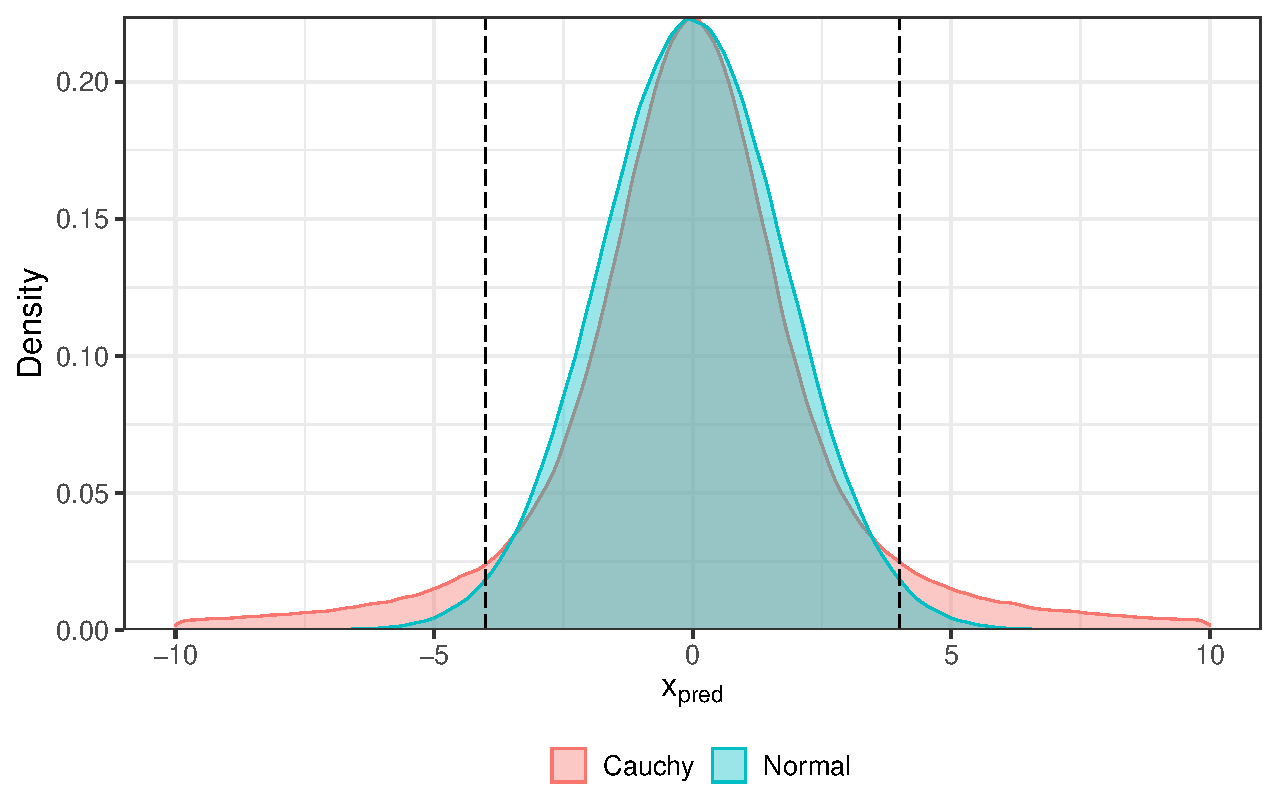
\includegraphics[scale=0.5]{figures/BC_example_326.pdf}
 \caption{Prior predictive distributions of $x$ under Normal and Cauchy priors.}
\end{figure}
\end{frame}
%%%%%%%%%%%%%%%%%%%%%%%%%%%%%%%%%%%
\begin{frame}{Conjugacy}
Conjugacy is a central concept in Bayesian statistics. 
It provides a functional view of the prior-posterior mechanic that emphasises tractability over coherence.
\begin{defn}[Conjugate]
\label{def:conjugate}
A family $\mathcal{F}$ of distributions on $\boldsymbol{\Theta}$ is called \textbf{conjugate} or closed under sampling for a likelihood $f(x \mid \theta)$ if, for every $\pi \in \mathcal{F}$, $p(\theta \mid x) \in \mathcal{F}$.
\end{defn}
\textbf{Arguments for using conjugate priors}
\begin{itemize}
 \item ``Form-preservation'': in a limited-information setting it makes sense that $p(\theta \mid x)$ and $\pi(\theta)$ lie on the same family, since the information in $x$ might not be enough to change the structure of the model, just its parameters;
 \item Simplicity: when you do not know a whole lot, it makes sense to KISS\footnote{Keep it simple, stupid!};
 \item Sequential learning: since $\mathcal{F}$ is closed under sampling, one can update a sequence of posteriors $p_i(\theta \mid x_1, \ldots, x_i)$ as data comes in.
\end{itemize}
\end{frame}
%%%%%%%%%%%%%%%%%%%%%%%%%%%%%%%%%%%
\begin{frame}{Exponential families}
The exponential family of distributions is a cornerstone of statistical practice, underlying many often-used models. 
Here are a few useful definitions.
\begin{defn}[(Natural) Exponential family]
 \label{def:expo_family}
 Let $\mu$ be a $\sigma$-finite measure on $\mathcal{X}$ and let $\boldsymbol{\Theta}$ be a non-empty set serving as the parameter space.
 Let $C : \boldsymbol{\Theta} \to (0, \infty)$ and $h: \boldsymbol{\Theta} \to (0, \infty)$ and let $R : \boldsymbol{\Theta} \times \mathcal{X} \to \mathbb{R}^k$ and $T: \boldsymbol{\Theta} \times \mathcal{X} \to \mathbb{R}^k$.
 The family of distributions with density 
 \begin{equation*}
  f(x \mid \theta) = C(\theta)h(x)\exp\left(R(\theta) \cdot T(x) \right)
 \end{equation*}
 w.r.t. $\mu$ is called an \textbf{exponential family}.
 Moreover, if $R(\theta) = \theta$, the family is said to be \textbf{natural}.
\end{defn}
\begin{defn}[Regular exponential family]
 We say a natural exponential family $f(x\mid\theta)$ is \textbf{regular} if the natural parameter space
 \begin{equation}
  N := \left\{ \theta : \int_{\mathcal{X}} \exp(\theta\cdot x) h(x)\,d\mu(x) < \infty \right\},
 \end{equation}
is an open set of the same dimension as the closure of the convex hull of $\supp(\mu)$.
\end{defn}
\end{frame}
%%%%%%%%%%%%%%%%%%%%%%%%%%%%%%%%%%%
\begin{frame}{Conjugacy and sufficiency}
There is an intimate link between sufficiency (i.e. the existence of sufficient statistics) and conjugacy.
The following is a staple of Bayesian theory.
\begin{theo}[Pitman-Koopman-Darmois]
 If a family of distributions $f(\cdot \mid \theta)$ whose support does not depend on $\theta$ is such that, for a sample size large enough, there exists a sufficient statistic of \underline{fixed dimension}, then $f(\cdot \mid \theta)$ is an exponential family.
\end{theo}
The support condition is not a complete deal breaker, however:
\begin{remark}[Quasi-exponential]
 The $\operatorname{Uniform}(-\theta, \theta)$ and $\operatorname{Pareto}(\theta, \alpha)$ families are called \textit{quasi-exponential} due to the fact that there do exist sufficient statistics of fixed dimension for these families, even though their supports depend on $\theta$.
\end{remark}
\end{frame}
%%%%%%%%%%%%%%%%%%%%%%%%%%%%%%%%%%%
\begin{frame}{Conjugacy in the exponential family}
I hope you are convinced of the utility of the exponential family by now.
It would be nice to have an automated way to deduce a conjugate prior for $f(x\mid \theta)$ when it is in the exponential family.
This is exactly what the next result gives us.
\begin{remark}[Conjugate prior for the exponential family]
 A conjugate family for $f(x\mid \theta)$ is given by
 \begin{equation}
 \label{eq:conjugate_exponential_family}
  \pi(\theta \mid \mu, \lambda) = K(\mu, \lambda) \exp\left(\theta \cdot \mu - \lambda g(\theta)\right),
 \end{equation}
such that the posterior is given by $p(\theta \mid \mu + x, \lambda + 1)$.
\end{remark}
Please do note that (\ref{eq:conjugate_exponential_family}) is only a valid density when $\lambda > 0$ and $\mu/\lambda$ belongs to the interior of the natural space parameter. 
Then, it is a $\sigma$-finite measure.
See \cite{Diaconis1979} for more details.
\end{frame}

%%%%%%%%%%%%%%%%%%%%%%%%%%%%%%%%%%%
\begin{frame}{Conjugacy: common families}
\begin{figure}
 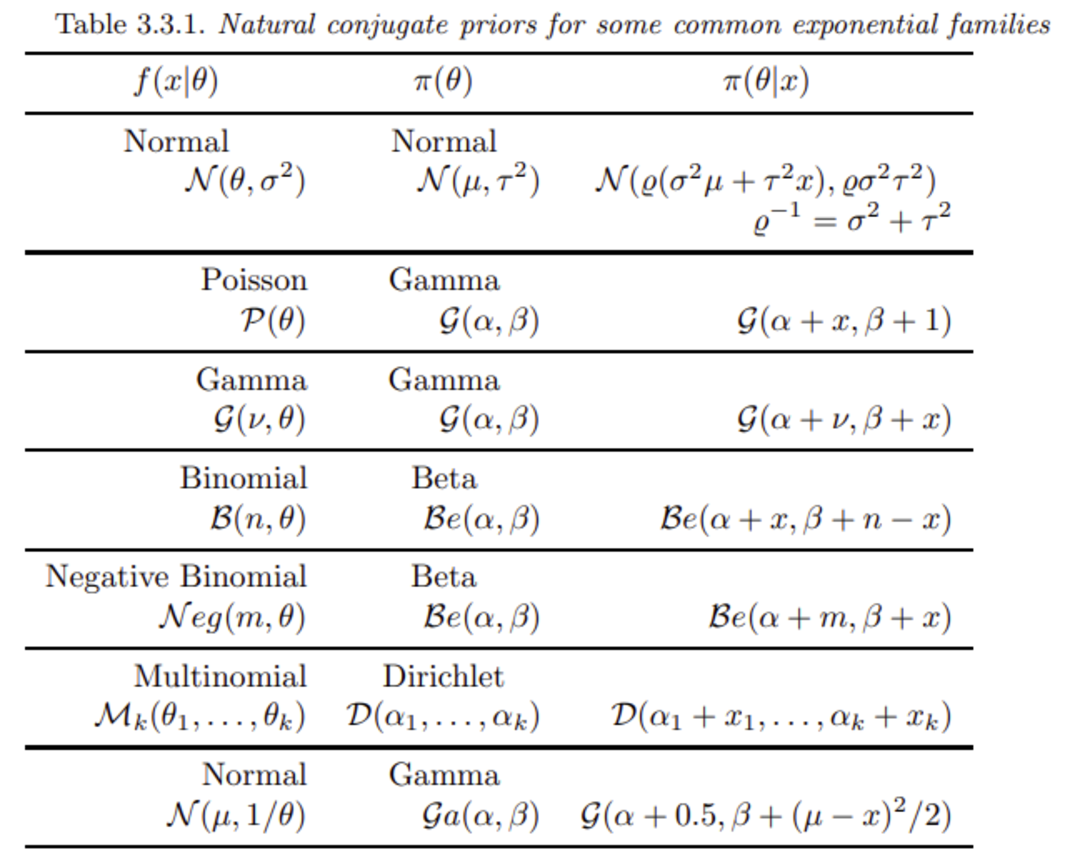
\includegraphics[scale=.5]{figures/conjugate_table.pdf}
 \caption{Taken from~\cite{Robert2007}, page 121.}
\end{figure}
\end{frame}
%%%%%%%%%%%%%%%%%%%%%%%%%%%%%%%%%%%
\begin{frame}{Conjugacy: drawbacks}
Conjugate modelling is certainly useful, but has its fair share of pitfalls.

\textbf{Arguments against using conjugate priors}
\begin{itemize}
 \item Conjugate priors are restrictive \textit{a priori}: in many settings, specially in high dimensions, the set of conjugate priors that retain tractability is so limited so as to not be able to encode all prior information available;
 \item Conjugate priors are not truly subjective: they limit the analyst's input to picking values for the hyperparameters;
  \item Conjugate priors are restrictive \textit{a posteriori}: you are stuck with a given structure forever, no matter how much data you run into.
\end{itemize}
\end{frame}
%%%%%%%%%%%%%%%%%%%%%%%%%%%%%%%%%%%
\begin{frame}{The principle of insufficient reason}
 Also called principle of indifference by Keynes\footnote{John Maynard Keynes (1883--1946) was an English economist.}.
 \begin{quote}
  ...if there is no known reason for predicating of our subject one rather than another of several alternatives, then relatively to such knowledge the assertions of each of these alternatives have an equal probability." \cite[Ch4 pg. 52-53]{Keynes1921}. 
 \end{quote}
 The idea dates back to Laplace and even Bayes himself and usually leads to 
$$ \pi(\theta) \propto 1.$$
 \end{frame}
%%%%%%%%%%%%%%%%%%%%%%%%%%%%%%%%%%%
\begin{frame}{Invariance}
In many applications we might want some sort of~\textit{invariance} in our prior model. 
\begin{defn}[Invariant model]
 \label{def:invariant_model}
 A statistical model is said to be~\textbf{invariant} (or closed) under the action of a group $\mathcal{G}$ if $\forall g \in \mathcal{G} \: \exists \theta^\star \in \boldsymbol{\Theta}$ such that $y = g(x)$ is distributed with density $f(y\mid \theta^\star)$, denoting $\theta^\star = \bar{g}(\theta)$.
\end{defn}
Consider two types of invariance
\begin{itemize}
 \item \textit{Translation} invariance:
 A model $f(x-\theta)$ such that $x-x_0$ has a distribution in the same family for every $x_0$ leads to
 $$\pi(\theta) = \pi(\theta-\theta_0),\: \forall\: \theta_0 \in \boldsymbol{\Theta}.$$
 \item \textit{Scale} invariance:
 Similarly, a model of the form $\sigma^{-1} f(x/\sigma)$, $\sigma >0$ is \textit{scale-invariant} and  leads to
 $$ \pi(A/c) = \pi(A),$$
 for any measurable A.
\end{itemize}
\end{frame}
%%%%%%%%%%%%%%%%%%%%%%%%%%%%%%%%%%
\begin{frame}{Jeffreys's prior}
One can try to build a prior that captures only the essential structural information about the problem by deriving an invariant distribution from the Fisher information:
$$ I(\theta) = E\left[\left(\frac{\partial \log f(X \mid \theta)}{\partial \theta}\right)^2\right].$$
Under regularity conditions, we can usually also write
$$ I(\theta) = - E\left[\frac{\partial^2 \log f(X \mid \theta)}{\partial \theta^2}\right].$$
Jeffreys showed that 
$$\pi_J(\theta) \propto \sqrt{I(\theta)},$$
is invariant.
There are straightforward generalisations when $\theta$ is multidimensional.
\end{frame}
%%%%%%%%%%%%%%%%%%%%%%%%%%%%%%%%%%
\begin{frame}{Jeffreys's priors: examples}
A good exercise is to show that
\begin{itemize}
 \item If $x \sim \operatorname{Normal}(0, \theta)$, $\pi_J(\theta) \propto 1/\theta^2$;
 \item If $x \sim \operatorname{Normal}_d(\theta, \boldsymbol{I}_d)$, $\pi_J(\theta) \propto 1$;
 \item If $x \sim \operatorname{Binomial}(n, \theta)$, $\pi_J(\theta) \equiv \operatorname{Beta}(1/2, 1/2)$;
 \item If $f(x\mid \theta) = h(x) \exp\left(\theta \cdot x - \psi(\theta)\right)$, then
 $$ \pi_J(\theta)  \propto \sqrt{\prod_{i=1}^k\psi^{\prime\prime}(\theta)}.$$
\end{itemize}
\end{frame}
%%%%%%%%%%%%%%%%%%%%%%%%%%%%%%%%%%
\begin{frame}{Beware!}
One important caveat of Jeffreys's priors is that they violate the Likelihood Principle.
To see why, consider the following exercise.
\begin{exercise}[Poisson process]
Suppose one is interested in estimating the rate, $\theta$, of a Poisson process:
$$ Y(t) \sim \operatorname{Poisson}(t\theta).$$
There are two possible experimental designs: 
\begin{itemize}
 \item[a)] Fix a number $n$ of events to be observed and record the time $X$ to observe them, or;
 \item[b)] Wait a fixed amount of time, $t$, and count the number $Y$ of occurences of the event of interest.
 Show that
\end{itemize}
 \begin{align*}
\label{eq:poisson_process_informationMatrix}
\text{a)}&\:  I_X(\theta) = \frac{n}{\theta^2},\\
\text{b)}&\: I_Y(\theta) = \frac{t}{\theta}.
\end{align*}
Which conclusions can we draw from this example?
\end{exercise}
See also example 3.5.7 in~\cite{Robert2007}.
\end{frame}
%%%%%%%%%%%%%%%%%%%%%%%%%%%%%%%%%%
\begin{frame}{Reference priors}
Jeffreys's approach can sometimes lead to marginalisation paradoxes and calibration issues (see exercise 4.47 in \cite{Robert2007}).
\cite{Bernardo1979} proposes a modification that avoids these difficulties by explicit separating parameters in~\textit{nuisance} and~\textit{interest}.
It works like this: take $f(x\mid \theta)$, with $\theta = (\theta_1, \theta_2)$ and let $\theta_1$ be the parameter of interest.
We must first compute\footnote{Notice that this need not be well-defined. One common way of dealing with difficulties is to integrate on a sequence of measurable compact sets and take the limit.}
$$ \tilde{f}(x\mid \theta_1) = \int_{\boldsymbol{\Theta_2}} f(x \mid \theta_1, t_2)\pi(t_2\mid \theta_1)\, dt_2, $$
and then compute the Jeffreys's prior associated with this marginalised likelihood.
Notice that this entails first deriving $\pi(\theta_2\mid \theta_1)$.
\end{frame}
%%%%%%%%%%%%%%%%%%%%%%%%%%%%%%%%%%
\begin{frame}{Reference priors: example}
Suppose we have $x_{ij} \sim \operatorname{Normal}(\mu_i, \sigma^2)$, $i = 1, \ldots, n$, $j=1,2$ and consider making inferences about $\boldsymbol{\theta} = (\sigma^2, \boldsymbol{\mu})$.
Here $\theta_1 = \sigma$ is a nuisance parameter and we're interested in the location $\boldsymbol{\theta}_2 = \boldsymbol{\mu}$.
The Jeffreys's prior is 
$$\pi_J(\boldsymbol{\theta}) \propto 1/\sigma^{n+1},$$
leading to a Bayes estimator under quadratic loss:
$$ \hat{\sigma}_J := E[\sigma^2 \mid \boldsymbol{x}] = \frac{\sum_{i=1}^n (x_{i1}-x_{i2})^2}{4n-4},$$
which in not consistent.
The reference approach give $\pi(\theta_1 \mid \boldsymbol{\theta_2})$ as a flat prior - because $\boldsymbol{\theta_2}$ is a location parameter.
Marginalising the likelihood against this flat density over $(0,\infty)$ gives $\pi_R(\sigma^2) \propto 1/\sigma^2$, leading to
$$ \hat{\sigma}_R =\frac{\sum_{i=1}^n (x_{i1}-x_{i2})^2}{2n-4},$$
which is consistent.
Phew!
\end{frame}
%%%%%%%%%%%%%%%%%%%%%%%%%%%%%%%%%%
\begin{frame}{Frequentist considerations}
If you are a bit greedy and want to please Greeks and Troyans, you might also try to construct your prior so that it attains good frequency properties. 
One such way is to construct~\textbf{matching priors}:
\begin{defn}[Matching prior]
 We say $\pi(\theta)$ is a \textbf{matching prior} for a confidence level $\alpha$ if it is constructed in such a way that  
 \begin{equation*}
  \pr(g(\theta) \in C_x \mid x) = \frac{1}{m(x)}\int_{C_x} f(x\mid t) \pi(t) \, dt = 1-\alpha,
 \end{equation*}
holds for a given confidence set $C_x(\alpha)$ for $g(\theta)$.
\end{defn}
In other words, if the posterior matches the confidence set.
It can be shown that, in unidimensional families, the Jeffreys's prior gives
$$ \pr(\theta \leq k_\alpha(x)) = 1-\alpha + O(n^{-1}),$$
where $C_x = (-\infty, k_\alpha(x))$ is a one-sided confidence interval.
\end{frame}
%%%%%%%%%%%%%%%%%%%%%%%%%%%%%%%%%%
\begin{frame}{Prior classes}
\cite{Robert2007} gives a classification of priors in classes:
\begin{itemize}
 \item[i)] Conjugate classes:
  $$ \Gamma_C = \{\pi \in \mathcal{F} : p \in \mathcal{F} \}, $$
 \item[ii)] Determined moment(s) classes:
 $$ \Gamma_M = \{\pi : a_i \leq E_\pi[\theta] \leq b_i, i = 1, \ldots, k\}, $$
 \item[iii)] Neighbourhood (or $\epsilon$-contamination) classes:
  $$ \Gamma_{\epsilon, \mathcal{Q}} = \{\pi = (1-\epsilon)\pi_0 + q, q \in \mathcal{Q}\}, $$
 \item[iv)] Underspecified classes:
   $$ \Gamma_{U} = \{\pi : \int_{I_i} \pi(t)\,dt \leq \mu_i, i = 1, \ldots, k\}, $$
 \item[v)] Ratio of density classes:
    $$ \Gamma_{R} = \{\pi : L(\theta) \leq \pi(\theta) \leq U(\theta)\}. $$
\end{itemize}
\end{frame}
%%%%%%%%%%%%%%%%%%%%%%%%%%%%%%%%%%
\begin{frame}{Prior sensitivity analysis}
 General recommendations about building priors:
 \begin{itemize}
  \item Check the \textbf{observable consequences} of your priors :what kinds of data does this produce?
  \item Check the inferential consequences of your priors: how do my estimators change under different priors?
  \item Make sure you know what your restrictions do to the tail of your prior;  
  \item It is usually a good idea to understand what the prior \textbf{does} to the model, as opposed to only which values $\theta$ can plausibly take;
  \item Sometimes it may be useful to think of priors as \textit{penalisations} that \textbf{regularise} inference.
 \end{itemize}
\end{frame}

%%%%%%%%%%%%%%%%%%%%%%%%%%%%%%%%%%
\begin{frame}{Recommended reading}
\begin{itemize}
 \item[\faBook] \cite{Robert2007} Ch. 3;
 \item[\faForward] Next lecture: \cite{Robert2007} Ch. 3.6, \cite{Seaman2012}, \cite{Gelman2017} and \cite{Simpson2017}.
 \end{itemize} 
\end{frame}

%%%%%%%
\begin{frame}[t, allowframebreaks]
\frametitle{References}
\bibliographystyle{apalike}
\bibliography{bayes}
\end{frame}
\end{document}
